\chapter{Principal Component Analysis}
\label{ch:pca}

\begin{chaptergoals}
\begin{itemize}[nosep]
\item A sample of vectors as a cloud of points in $\real^d$: its mean vector and covariance matrix, and the sample variance of the cloud in a direction $u$, which is $u^\top Su$.
\item The direction of greatest spread is the first eigenvector of $S$, the next the second, and so on: the principal directions, proved from the spectral theorem.
\item Principal component analysis as the best flat picture of the cloud: the projection onto the first $k$ principal directions loses less than any other $k$-dimensional projection, and the eigenvalues say how much.
\item What the sample covariance estimates: $S \convp \Sigma$ entry by entry by the Law of Large Numbers, and the sample directions converge to the population's by the continuous mapping theorem. The units pitfall, and what happens when $d$ is not small against $n$.
\end{itemize}
Every chapter so far had one variable to explain or one parameter to estimate. This last chapter looks at many variables at once with no one of them singled out, and asks only in which directions they vary together.
\end{chaptergoals}

\section{A cloud of points}
\label{sec:pca-cloud}

The Old Faithful record of \cref{ch:regression-uni} has two numbers per eruption, its duration and the wait to the next one; the stack loss record of \cref{ch:regression-multi} has four per day.
Regression picked one of them as the response.
Drop that choice: each observation is a point $X_i \in \real^d$, the sample is a cloud of $n$ points, and the question is the cloud's shape.

\begin{definition}[Mean vector and covariance matrix]
\label{def:covmatrix}
Let $X = (X^{(1)}, \ldots, X^{(d)})^\top$ be a random vector with $\E[\norm{X}^2] < \infty$.
Its \textbf{mean vector} is $\E[X] = (\E[X^{(1)}], \ldots, \E[X^{(d)}])^\top$ and its \textbf{covariance matrix} is the $d \times d$ matrix
\[
\Sigma = \E\big[(X - \E[X])(X - \E[X])^\top\big], \qquad \Sigma_{jk} = \cov(X^{(j)}, X^{(k)}),
\]
with the variances on the diagonal.
For a sample $X_1, \ldots, X_n$ the \textbf{sample mean vector} is $\bar{X} = \frac1n\sum_i X_i$ and the \textbf{sample covariance matrix} is
\[
S = \frac1n\sum_{i=1}^n (X_i - \bar{X})(X_i - \bar{X})^\top,
\]
whose $(j, k)$ entry is the sample covariance of the $j$th and $k$th coordinates, with divisor $n$.
\end{definition}

\begin{inwords}
The mean vector is the center of the cloud and the covariance matrix its shape: each diagonal entry is the spread along one axis, each off-diagonal entry says whether two coordinates move together. The sample versions are the same averages over the points. With $\mathbf{X}$ the $n \times d$ matrix whose rows are the $X_i^\top$ (the design matrix of \cref{ch:regression-multi}, in bold here because $X$ is the random vector), $\bar{X} = \frac1n\mathbf{X}^\top\mathbf{1}$ and $S = \frac1n\mathbf{X}^\top H\mathbf{X}$ with $H = I - \frac1n\mathbf{1}\mathbf{1}^\top$ the projection that removes the column means.

\textbf{For the kiss data.} With $d = 1$ the vector is the single $0/1$ variable $R_i$, the mean vector is $\hat{p} = 0.645$ and the covariance matrix is the one number $\hat{p}(1 - \hat{p}) = 0.229$, the sample variance with divisor $n$ (\cref{ch:estimators}). For Old Faithful, $d = 2$: the mean vector is $(3.49, 70.9)$ and
\[
S = \begin{pmatrix} 1.30 & 13.9 \\ 13.9 & 184.1 \end{pmatrix},
\]
a duration variance of $1.30$ minutes squared, a waiting variance of $184$, and a covariance of $13.9$, which is the correlation $r = 0.90$ of \cref{ch:regression-uni} times the two standard deviations.
\end{inwords}

The one fact about $S$ the chapter runs on is what it says about a direction.

\begin{proposition}[Variance in a direction]
\label{prop:pca-direction}
For any $u \in \real^d$, $u^\top\Sigma u = \var(u^\top X)$, and $u^\top Su$ is the sample variance, with divisor $n$, of the $n$ numbers $u^\top X_1, \ldots, u^\top X_n$.
Both matrices are symmetric and positive semidefinite.
If $u^\top Su = 0$ then every $X_i$ lies in the hyperplane $\{x : u^\top x = u^\top\bar{X}\}$.
\end{proposition}
\optionalproof{Pull the fixed vector $u$ out of the expectation or the average: $u^\top(X - \E X)(X - \E X)^\top u = (u^\top(X - \E X))^2$.}
\begin{proof}
$u^\top\Sigma u = \E[u^\top(X - \E[X])(X - \E[X])^\top u] = \E[(u^\top X - u^\top\E[X])^2] = \var(u^\top X)$, since $u^\top\E[X] = \E[u^\top X]$; likewise $u^\top Su = \frac1n\sum_i(u^\top X_i - u^\top\bar{X})^2$, and $u^\top\bar{X}$ is the mean of the $u^\top X_i$.
A variance is non-negative, so both matrices are positive semidefinite, and they are symmetric because $\cov(X^{(j)}, X^{(k)}) = \cov(X^{(k)}, X^{(j)})$.
If the sample variance of the $u^\top X_i$ is $0$ they all equal their mean $u^\top\bar{X}$.
\end{proof}

For a unit vector $u$, the $u^\top X_i$ are the coordinates of the points along the axis through the origin in direction $u$, so $u^\top Su$ is how far the cloud spreads along that axis, and the proposition turns a question about the cloud into a question about one matrix.
\Cref{fig:pcadirection} plots $u^\top Su$ against the angle of $u$ for the Old Faithful cloud after each variable has been standardized (write $Z_i$ for the standardized $X_i$, with coordinates $z_{i1}, z_{i2}$: each coordinate is centered and divided by its standard deviation, so that $S$ becomes the correlation matrix, with $1$s on the diagonal and $r = 0.90$ off it): the spread is $1 + 0.90\sin 2t$ at angle $t$, largest along the diagonal at $45^\circ$, where it is $1.90$, and smallest at $135^\circ$, where it is $0.10$, with the two extremes at right angles.
Which directions those are, and why they are perpendicular, is the subject of the next section.

\begin{figure}[htbp]
\centering
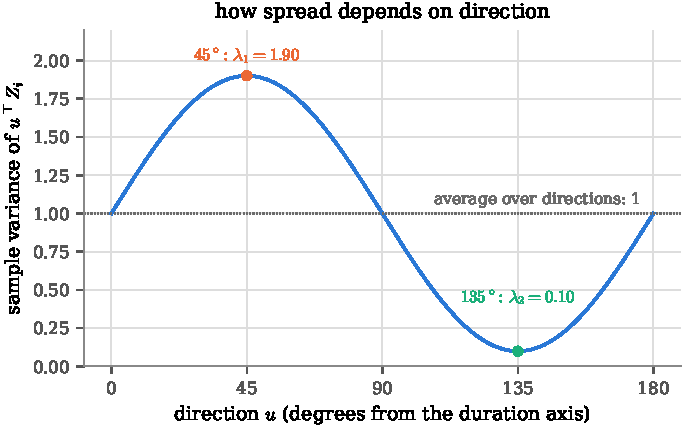
\includegraphics[width=0.78\textwidth]{fig_pca_direction}
\caption{The sample variance of $u^\top Z_i$ for the standardized Old Faithful data against the angle of the unit vector $u$: $1 + 0.90\sin 2t$, with its maximum $1.90$ at $45^\circ$ and its minimum $0.10$ at $135^\circ$.}
\label{fig:pcadirection}
\end{figure}

\section{The principal directions}
\label{sec:pca-directions}

$S$ is symmetric, so the spectral theorem \toolkit{sec:math-eigen} writes it as
\[
S = PDP^\top = \sum_{j=1}^d \lambda_jv_jv_j^\top, \qquad \lambda_1 \geq \lambda_2 \geq \cdots \geq \lambda_d \geq 0,
\]
with $P = (v_1, \ldots, v_d)$ orthogonal, so the $v_j$ are orthonormal, and the eigenvalues non-negative because $S$ is positive semidefinite.
The theorem of this chapter says the eigenvectors are the directions the cloud spreads along and the eigenvalues are the spreads.

\begin{theorem}[Principal directions]
\label{thm:pca-directions}
Let $S = PDP^\top$ as above. Then:
\begin{enumerate}[nosep]
\item $v_1$ maximizes $u^\top Su$ over unit vectors $u$, and the maximum is $\lambda_1$;
\item for $j = 2, \ldots, d$, $v_j$ maximizes $u^\top Su$ over unit vectors perpendicular to $v_1, \ldots, v_{j-1}$, and the maximum is $\lambda_j$;
\item the sample covariance matrix of the rotated points $P^\top X_i$ is $D$: the coordinates along the $v_j$ have sample variances $\lambda_j$ and sample covariances $0$; and $\sum_j\lambda_j = \mathrm{tr}(S)$, the sum of the $d$ sample variances.
\end{enumerate}
\end{theorem}
\coreproof{In the eigenvector coordinates $c = P^\top u$, the quadratic form is $\sum_j\lambda_jc_j^2$ with $\sum_jc_j^2 = 1$: a weighted average of the eigenvalues, largest when all the weight sits on the largest one. Perpendicularity to the first $j - 1$ eigenvectors sets their coordinates to zero, and the same argument runs on the rest.}
\begin{proof}
For a unit vector $u$ put $c = P^\top u$, so $u = Pc$ and $\norm{c}^2 = c^\top P^\top Pc = \norm{u}^2 = 1$.
Then $u^\top Su = c^\top P^\top PDP^\top Pc = c^\top Dc = \sum_j\lambda_jc_j^2 \leq \lambda_1\sum_jc_j^2 = \lambda_1$, with equality when $c = e_1$, that is, $u = v_1$: this is (1).
If $u$ is perpendicular to $v_1, \ldots, v_{j-1}$ then $c_1 = \cdots = c_{j-1} = 0$, since $c_k = v_k^\top u$, so $u^\top Su = \sum_{k \geq j}\lambda_kc_k^2 \leq \lambda_j$, with equality at $u = v_j$: this is (2).
For (3), the rotated points have mean $P^\top\bar{X}$ and sample covariance $\frac1n\sum_iP^\top(X_i - \bar{X})(X_i - \bar{X})^\top P = P^\top SP = D$; and $\mathrm{tr}(S) = \mathrm{tr}(PDP^\top) = \mathrm{tr}(DP^\top P) = \mathrm{tr}(D)$.
\end{proof}

\begin{definition}[Principal directions and components]
\label{def:pca}
The eigenvectors $v_1, \ldots, v_d$ of $S$, ordered by decreasing eigenvalue, are the sample's \textbf{principal directions}; the numbers $v_j^\top(X_i - \bar{X})$, $i = 1, \ldots, n$, are its $j$th \textbf{principal component} (or \textbf{scores}); and $\lambda_j/\mathrm{tr}(S)$ is the \textbf{proportion of the variance explained} by the $j$th component.
\end{definition}

\begin{inwords}
Rotate the axes so that the first points along the cloud's longest extent, the second along the longest extent perpendicular to it, and so on. In the new axes the coordinates are uncorrelated, their variances are the eigenvalues, and the total variance is the same as before, since a rotation does not change distances. The scores are the coordinates of each point in the new axes, measured from the center.

\textbf{For the kiss data.} With one variable there is one direction and nothing to rotate. For the standardized Old Faithful data (\cref{fig:pcacloud}), $v_1 = (0.71, 0.71)$ and $v_2 = (-0.71, 0.71)$ with $\lambda_1 = 1.90$ and $\lambda_2 = 0.10$: the first component is $(z_{i1} + z_{i2})/\sqrt2$, an eruption's size on the two measures combined, and carries $1.90/2 = 95\%$ of the variance; the second is $(z_{i2} - z_{i1})/\sqrt2$, how far the standardized wait sits above the standardized duration, and carries $5\%$.
\end{inwords}

\begin{figure}[htbp]
\centering
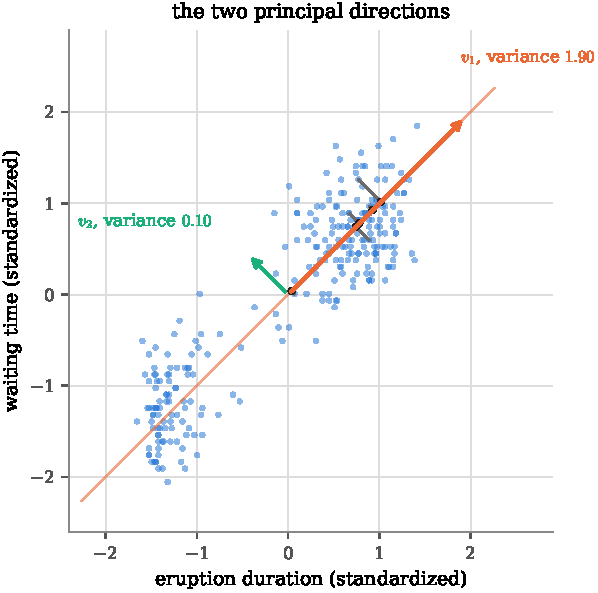
\includegraphics[width=0.6\textwidth]{fig_pca_cloud}
\caption{The standardized Old Faithful cloud with the line along its first principal direction, the two principal directions from the mean, each drawn with length $2\sqrt{\lambda_j}$, and five points of the upper cluster projected onto the first (gray segments, black dots).}
\label{fig:pcacloud}
\end{figure}

A correlation matrix with $1$s on the diagonal and $r$ off it always has eigenvectors $(1, 1)/\sqrt2$ and $(-1, 1)/\sqrt2$ with eigenvalues $1 + r$ and $1 - r$ (\cref{ex:pca-twobytwo}), so for two standardized variables the principal directions are the two diagonals whatever the data, the rising one first when $r > 0$, and only the eigenvalues carry information.
With more variables the directions are no longer fixed in advance, and they are what the method is for.
The method is Pearson's (1901), who found the line and the plane of closest fit to a cloud of points, which is \cref{thm:pca-projection} below; Hotelling (1933) named the principal components and tied them to the eigenvectors of the covariance matrix.

\begin{pitfall}[units decide the directions]
$u^\top Su$ is a variance, in the units of $u^\top X$, and changing the unit of one coordinate changes the eigenvectors, not just the eigenvalues. \Cref{fig:pcaunits} shows Old Faithful in its raw units, duration in minutes with variance $1.30$ and waiting in minutes with variance $184$: the first principal direction is tilted $86^\circ$ toward the waiting axis and explains $99.9\%$ of the variance, which says only that $184$ is much larger than $1.30$. Measure the duration in seconds instead and the picture tilts the other way. When the coordinates are measured in different units, or in the same unit on very different scales, standardize them first; the analysis is then of the correlation matrix, and the first direction is the one along which the standardized variables move together most. When the coordinates share a unit and their scales mean something, as with $d$ measurements of the same kind, the raw covariance matrix is the right object.
\end{pitfall}

\begin{figure}[htbp]
\centering
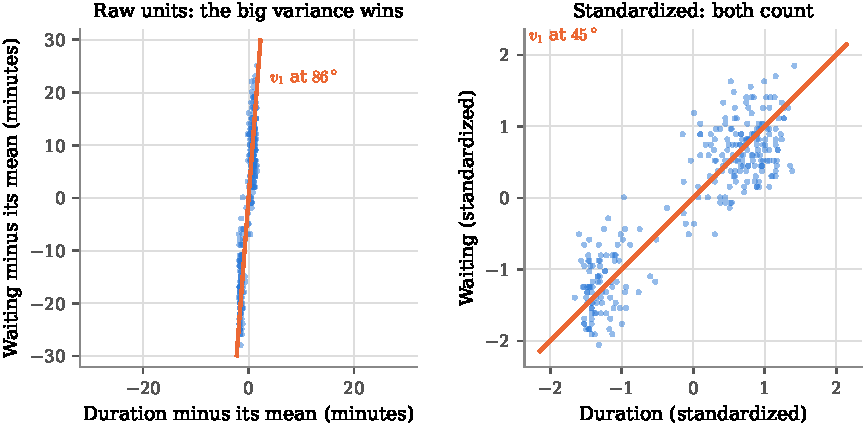
\includegraphics[width=\textwidth]{fig_pca_units}
\caption{Old Faithful with both axes in minutes (left, equal scales) and standardized (right). The first principal direction (orange) follows the variable with the larger variance on the left and the diagonal on the right.}
\label{fig:pcaunits}
\end{figure}

\section{The best flat picture}
\label{sec:pca-projection}

A cloud in $\real^d$ with $d > 3$ cannot be drawn.
Principal component analysis draws it anyway, by projecting it onto the plane (or the line, or a $k$-dimensional subspace) along which it is most spread out, and the point of the next theorem is that the plane which keeps the most variance is also the plane which loses the least distance.

\begin{theorem}[Projection onto the first $k$ principal directions]
\label{thm:pca-projection}
Let $S = PDP^\top$ as above, let $1 \leq k < d$, and for an orthonormal $u_1, \ldots, u_k$ let $Q$ be the projection onto their span, $Qx = \sum_{j \leq k}(u_j^\top x)u_j$.
Over all such choices, the sum of squared distances from the centered points to their projections,
\[
\sum_{i=1}^n\norm{(X_i - \bar{X}) - Q(X_i - \bar{X})}^2 = n\Big(\mathrm{tr}(S) - \sum_{j=1}^k u_j^\top Su_j\Big),
\]
is smallest when $u_1, \ldots, u_k$ span the same subspace as $v_1, \ldots, v_k$, and its minimum is $n(\lambda_{k+1} + \cdots + \lambda_d)$.
The projected cloud then has total variance (the sum of its $k$ sample variances) $\lambda_1 + \cdots + \lambda_k$, a proportion $(\lambda_1 + \cdots + \lambda_k)/\mathrm{tr}(S)$ of $\mathrm{tr}(S)$, the cloud's total.
\end{theorem}
\coreproof{Pythagoras splits each centered point's squared length into the part along the subspace and the part lost; summing, the lost part is the total variance minus the variance kept, $\sum_{j \leq k}u_j^\top Su_j$. Keeping the most is choosing $k$ orthonormal directions whose quadratic forms add up to the most, and in eigenvector coordinates that sum is $\sum_j\lambda_jw_j$ with weights $w_j \in [0, 1]$ adding up to $k$, which is largest with the weight on the $k$ largest eigenvalues.}
\begin{proof}
Write $Y_i = X_i - \bar{X}$.
Since $Q$ is an orthogonal projection, $\norm{Y_i}^2 = \norm{QY_i}^2 + \norm{Y_i - QY_i}^2$ \toolkit{sec:math-matrices}, and $\norm{QY_i}^2 = \sum_{j \leq k}(u_j^\top Y_i)^2$ by orthonormality.
Summing over $i$ and dividing by $n$, $\frac1n\sum_i\norm{Y_i}^2 = \mathrm{tr}(S)$ (the sum of the $d$ sample variances) and $\frac1n\sum_i(u_j^\top Y_i)^2 = u_j^\top Su_j$ (\cref{prop:pca-direction}, the $u_j^\top Y_i$ having mean $0$), which gives the displayed identity.
It remains to maximize $\sum_{j \leq k}u_j^\top Su_j$.
Put $c_j = P^\top u_j$, orthonormal since $P$ is orthogonal, so that $u_j^\top Su_j = \sum_m\lambda_mc_{jm}^2$ and
\[
\sum_{j=1}^k u_j^\top Su_j = \sum_{m=1}^d\lambda_mw_m, \qquad w_m = \sum_{j=1}^k c_{jm}^2.
\]
Each $w_m \leq 1$, since $c_{1m}, \ldots, c_{km}$ are the $m$th coordinates of $k$ orthonormal vectors, which extend to an orthonormal basis of $\real^d$, whose $m$th coordinates have squares summing to $1$ \toolkit{sec:math-gaussvec}; and $\sum_mw_m = \sum_j\norm{c_j}^2 = k$.
A sum $\sum_m\lambda_mw_m$ with $\lambda_1 \geq \cdots \geq \lambda_d$, $0 \leq w_m \leq 1$ and $\sum_mw_m = k$ is at most $\lambda_1 + \cdots + \lambda_k$: moving weight from any $m > k$ to any $m' \leq k$ with $w_{m'} < 1$ cannot decrease it, and when no such move is left the weights are $1$ on $m \leq k$ and $0$ after.
The bound is attained by $u_j = v_j$, where $c_j = e_j$; and any orthonormal $u_1, \ldots, u_k$ spanning the same subspace give the same projection $Q$, hence the same loss.
\end{proof}

\begin{inwords}
Among all flat pictures of dimension $k$, the one drawn on the first $k$ principal directions is the one in which the points move least from where they were, and what it loses is exactly the sum of the eigenvalues it leaves out. The proportion of the variance explained says how much of the cloud's variance the picture keeps.

\textbf{For the kiss data.} With $d = 1$ there is nothing to project. The standardized Old Faithful cloud projected onto $v_1$ (\cref{fig:pcacloud}) keeps $95\%$ of its variance, and the squared distances the points move add up to $n\lambda_2 = 272 \times 0.10 = 27$.
\end{inwords}

In practice the analysis runs in three steps: center the data (and standardize them unless the units agree), compute the eigenvectors and eigenvalues of $S$, and choose $k$.
The choice of $k$ is a judgment with two common guides.
The \textbf{scree plot} draws $\lambda_j$ against $j$ and stops where the fall flattens, the eigenvalues past that point being read as noise; the \textbf{proportion explained} chooses the smallest $k$ with $(\lambda_1 + \cdots + \lambda_k)/\mathrm{tr}(S)$ above a threshold such as $0.9$.
For a picture, $k$ is $2$ or $3$ whatever the eigenvalues say.

\begin{worked}[the stack loss data in four dimensions]
The $21$ days of \cref{ch:regression-multi} have four measurements each, air flow, water temperature, acid concentration and stack loss, in different units, so the analysis is of the correlation matrix, whose off-diagonal entries are $0.78$ (air, water), $0.50$ (air, acid), $0.92$ (air, loss), $0.39$ (water, acid), $0.88$ (water, loss) and $0.40$ (acid, loss). Its eigenvalues are $3.00$, $0.73$, $0.22$ and $0.05$, which explain $75\%$, $18\%$, $5\%$ and $1\%$ of the variance (\cref{fig:pcascree}): two components keep $93\%$. The first direction is $v_1 = (0.55, 0.52, 0.35, 0.55)$, close to an equal-weight average of the four standardized variables, an overall `how hard the plant was running' score, on which days $1$ to $3$ sit far to the right and days $17$ to $19$ far to the left. The second, $v_2 = (-0.08, -0.26, 0.93, -0.26)$, is the acid concentration against everything else: acid is the variable least tied to the other three (its correlations are $0.39$ to $0.50$), and the second component separates days by it, day $14$ at the top and day $17$ at the bottom. The regression of \cref{ch:regression-multi} explained the loss by the other three; the first component says the three and the loss mostly rise and fall together.
\end{worked}

\begin{figure}[htbp]
\centering
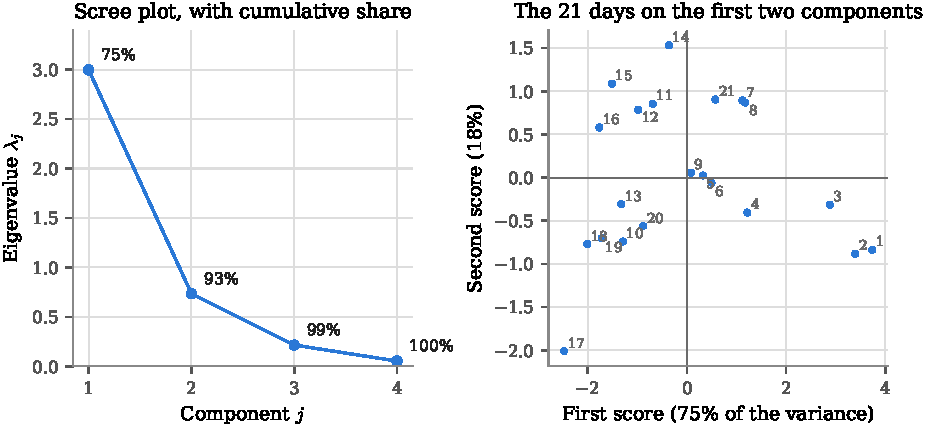
\includegraphics[width=\textwidth]{fig_pca_scree}
\caption{Stack loss, four standardized variables. Left: the scree plot of the eigenvalues $3.00$, $0.73$, $0.22$, $0.05$ with the cumulative share explained. Right: the $21$ days on their first two principal components, numbered.}
\label{fig:pcascree}
\end{figure}

\section{What the sample directions estimate}
\label{sec:pca-estimation}

Everything so far was a description of $n$ points, with no model behind it, and principal component analysis is used in that spirit on clouds that are not random at all.
When the $X_i$ are i.i.d.\ copies of a random vector $X$, the sample quantities estimate population ones, and the book's limit theorems say in what sense.

\begin{theorem}[Consistency of the sample covariance and its eigenvectors]
\label{thm:pca-consistent}
Let $X_1, X_2, \ldots$ be i.i.d.\ copies of $X \in \real^d$ with $\E[\norm{X}^4] < \infty$, mean $m$ and covariance matrix $\Sigma$, with eigenvalues $\lambda_1^* \geq \cdots \geq \lambda_d^*$ and orthonormal eigenvectors $v_1^*, \ldots, v_d^*$.
Then:
\begin{enumerate}[nosep]
\item $\bar{X} \convp m$ and $S \convp \Sigma$, entry by entry;
\item each sample eigenvalue converges: $\lambda_j \convp \lambda_j^*$ for $j = 1, \ldots, d$;
\item if $\lambda_j^*$ differs from both its neighbors, $\lambda_{j-1}^* > \lambda_j^* > \lambda_{j+1}^*$ (only the second inequality when $j = 1$, only the first when $j = d$), the sample direction converges to the population direction: with the signs chosen so that $v_j^\top v_j^* \geq 0$, $v_j \convp v_j^*$.
\end{enumerate}
\end{theorem}
\coreproof{Each entry of $S$ is an average of products of coordinates minus a product of averages, so the Law of Large Numbers and the continuous mapping theorem give (1); the eigenvalues, and the eigenvector lines where the eigenvalue is isolated, are continuous functions of the matrix, so the continuous mapping theorem gives (2) and (3).}
\recall{The Law of Large Numbers (\cref{thm:wlln}): for i.i.d.\ $Z_i$ with $\var(Z_i) < \infty$, $\frac1n\sum_iZ_i \convp \E[Z_i]$. The continuous mapping theorem (\cref{thm:cmt}): if $Y_n \convp y$ and $f$ is continuous, then $f(Y_n) \convp f(y)$; it holds for a vector $Y_n \convp y$ and a continuous $f$ of several variables, since continuity of $f$ at $y$ gives a $\delta$ with $\norm{f(z) - f(y)} \leq \epsilon$ whenever $\norm{z - y} \leq \delta$, so $\Pr(\norm{f(Y_n) - f(y)} > \epsilon) \leq \Pr(\norm{Y_n - y} > \delta) \to 0$; and a vector converges in probability as soon as each of its $q$ coordinates does, since $\Pr(\norm{Y_n - y} > \epsilon) \leq \sum_{j=1}^q\Pr(\abs{Y_n^{(j)} - y_j} > \epsilon/\sqrt{q})$.}
\begin{proof}
Write $S = \frac1n\sum_iX_iX_i^\top - \bar{X}\bar{X}^\top$ (expand the square in \cref{def:covmatrix}).
The $(j, k)$ entry of the first term is the average of the i.i.d.\ products $X_i^{(j)}X_i^{(k)}$, whose variance is finite by the fourth-moment assumption, so it converges in probability to $\E[X^{(j)}X^{(k)}]$; and $\bar{X}^{(j)} \convp m_j$ by the Law of Large Numbers with the second moments finite.
Since the vector of all $d + d^2$ quantities then converges in probability (each coordinate does), and $(a, b) \mapsto a - bb^\top$ is continuous, the continuous mapping theorem gives $S \convp \E[XX^\top] - mm^\top = \Sigma$ entry by entry, which is (1).
The map from a symmetric matrix to its $j$th largest eigenvalue is continuous \toolkit{sec:math-eigen}, so (2) follows from (1) by the continuous mapping theorem; and where $\lambda_j^*$ is isolated from its neighbors, the map to the unit eigenvector with the sign fixed by $v_j^\top v_j^* \geq 0$ is continuous at $\Sigma$, which gives (3) (the map need only be continuous where the limit lives, as \cref{ch:limit-tools} notes).
\end{proof}

The condition in (3) is not decoration: when two population eigenvalues are equal, any direction in the plane they span is an eigenvector, and the sample direction wanders in that plane however large $n$ is.
For the standardized Old Faithful data, the gap $1.90$ against $0.10$ is wide, and the sample directions are the population's diagonals in any case.
There is a Central Limit Theorem to go with the Law: for Gaussian data, $\sqrt{n}(\lambda_j - \lambda_j^*) \convd \Gauss(0, 2\lambda_j^{*2})$ when $\lambda_j^*$ is isolated (Anderson, 1963), so a sample eigenvalue has a standard error of about $\lambda_j\sqrt{2/n}$; it is stated here and not proved, and nothing depends on it.

\begin{pitfall}[many variables, few observations]
The theorem lets $n$ grow with $d$ fixed. When $d$ is comparable to $n$, or larger, $S$ is a poor estimate of $\Sigma$ even though each of its entries is consistent: with $d > n$ the cloud spans at most $n - 1$ dimensions, $S$ has rank at most $n - 1$, and at least $d - n + 1$ of its eigenvalues are exactly $0$ whatever $\Sigma$ is. The largest sample eigenvalue is then biased upward and the smallest downward, and the first sample direction can be far from $v_1^*$ even when the gap below $\lambda_1^*$ is wide. Gene expression data, with thousands of genes measured on hundreds of people, are the standard case. The remedies assume something about $\Sigma$: that it has low rank, so that only the first $k$ sample components are kept and the rest treated as noise, or that $v_1^*$ has few nonzero coordinates (sparse principal components), both outside this book.
\end{pitfall}

\section{Where the book ends}
\label{sec:pca-end}

The book began with $124$ couples and one proportion, and it ends with $21$ days and a four-by-four matrix, but the tools did not change.
A model says what the data could have been; an estimator is a function of the data; the Law of Large Numbers says it settles down, the Central Limit Theorem says how, and Slutsky, the continuous mapping theorem and the delta method carry those two facts to every estimator built from averages, which is nearly all of them.
Maximum likelihood turned those tools into a method, with the Fisher information as its yardstick; tests and intervals were the same calculation read two ways; the Bayesian chapters put a prior on the parameter and found, in large samples, the same answers; regression and its generalizations put a linear predictor behind the mean; and this chapter dropped the response and kept the covariance.
What comes after, in the next book of the series, is the same tools, the theorems of \cref{ch:lln,ch:clt,ch:limit-tools}, applied to harder models.

\section{Summary}
\label{sec:pca-summary}

\begin{itemize}[nosep]
\item A sample of vectors is a cloud in $\real^d$ with mean vector $\bar{X}$ and sample covariance matrix $S = \frac1n\sum_i(X_i - \bar{X})(X_i - \bar{X})^\top$; $u^\top Su$ is the cloud's variance along $u$. Old Faithful: variances $1.30$ and $184$, covariance $13.9$, correlation $0.90$.
\item Spectral theorem: $S = PDP^\top$ with orthonormal eigenvectors and eigenvalues $\lambda_1 \geq \cdots \geq \lambda_d \geq 0$. The eigenvectors are the principal directions: $v_1$ maximizes $u^\top Su$ with value $\lambda_1$, $v_j$ does so among directions perpendicular to the earlier ones, the rotated coordinates are uncorrelated with variances $\lambda_j$, and $\sum_j\lambda_j = \mathrm{tr}(S)$.
\item Projecting onto the first $k$ principal directions loses $n(\lambda_{k+1} + \cdots + \lambda_d)$ in squared distance, less than any other $k$-dimensional projection, and keeps the proportion $(\lambda_1 + \cdots + \lambda_k)/\mathrm{tr}(S)$ of the variance. Choose $k$ by the scree plot or a proportion threshold. Stack loss: $75\%$, $93\%$, $99\%$, with an overall-activity first direction and an acid-against-the-rest second.
\item Standardize when the units differ: in raw minutes Old Faithful's first direction is at $86^\circ$ and explains $99.9\%$, which only reports the ratio of two variances.
\item With i.i.d.\ data and fourth moments, $S \convp \Sigma$ entry by entry (LLN and CMT), the eigenvalues converge, and each eigenvector converges where its eigenvalue is isolated. For Gaussian data $\sqrt{n}(\lambda_j - \lambda_j^*) \convd \Gauss(0, 2\lambda_j^{*2})$ (stated). With $d$ near or above $n$ the sample eigenvalues are badly biased and extra assumptions are needed.
\end{itemize}

\section{Exercises}
\label{sec:pca-exercises}

\begin{exercise}
\label{ex:pca-twobytwo}
(a) Show that $\begin{pmatrix} 1 & r \\ r & 1\end{pmatrix}$ has eigenvectors $(1, 1)/\sqrt2$ and $(-1, 1)/\sqrt2$ with eigenvalues $1 + r$ and $1 - r$, and check the Old Faithful values $1.90$ and $0.10$. (b) Show that for the unit vector $u = (\cos t, \sin t)$, $u^\top Su = 1 + r\sin 2t$, the curve of \cref{fig:pcadirection}, and find its average over $t$. (c) For a general $2 \times 2$ covariance matrix $\begin{pmatrix} a & c \\ c & b\end{pmatrix}$, show that the first principal direction makes the angle $\frac12\arctan\big(2c/(a - b)\big)$ with the first axis (when $a > b$; when $a < b$ the maximum is at the other root of $\tan 2t = 2c/(a - b)$, $90^\circ$ away), and compute it for Old Faithful's raw $S$.
\end{exercise}
\begin{solution}
(a) $\begin{pmatrix} 1 & r \\ r & 1\end{pmatrix}\begin{pmatrix} 1 \\ 1\end{pmatrix} = (1 + r)\begin{pmatrix} 1 \\ 1\end{pmatrix}$ and likewise $(1 - r)$ for $(-1, 1)$; with $r = 0.90$, $1.90$ and $0.10$. (b) $u^\top Su = \cos^2t + \sin^2t + 2r\sin t\cos t = 1 + r\sin 2t$; its average over a full turn is $1$, the average of the eigenvalues, that is, $\mathrm{tr}(S)/d$. (c) $u^\top Su = a\cos^2t + b\sin^2t + 2c\sin t\cos t = \frac{a + b}{2} + \frac{a - b}{2}\cos 2t + c\sin 2t$, whose derivative in $t$ vanishes when $\tan 2t = 2c/(a - b)$. For Old Faithful $a < b$, and $2 \times 13.9/(1.30 - 184.1) = -0.152$ gives $2t = -8.6^\circ$ for the minimum and $2t = 180^\circ - 8.6^\circ$ for the maximum, so $t = 85.7^\circ$, the $86^\circ$ of \cref{fig:pcaunits}.
\end{solution}

\begin{exercise}
\label{ex:pca-projector}
Let $H = I - \frac1n\mathbf{1}\mathbf{1}^\top$ with $\mathbf{1} \in \real^n$ the vector of ones. Show that $H$ is symmetric with $H^2 = H$, say onto which subspace it projects, and verify $S = \frac1n\mathbf{X}^\top H\mathbf{X}$ for the $n \times d$ data matrix $\mathbf{X}$.
\end{exercise}
\begin{solution}
$H^\top = H$ is clear, and $H^2 = I - \frac2n\mathbf{1}\mathbf{1}^\top + \frac{1}{n^2}\mathbf{1}(\mathbf{1}^\top\mathbf{1})\mathbf{1}^\top = I - \frac1n\mathbf{1}\mathbf{1}^\top = H$ since $\mathbf{1}^\top\mathbf{1} = n$. $H\mathbf{1} = 0$ and $Hv = v$ for $v \perp \mathbf{1}$, so $H$ projects onto the vectors with coordinates summing to $0$, the orthogonal complement of the line through $\mathbf{1}$ (the residual projection of \cref{ch:regression-multi} for the intercept-only model). $H\mathbf{X}$ subtracts each column's mean from the column, so its rows are $(X_i - \bar{X})^\top$, and $\frac1n\mathbf{X}^\top H\mathbf{X} = \frac1n(H\mathbf{X})^\top(H\mathbf{X}) = \frac1n\sum_i(X_i - \bar{X})(X_i - \bar{X})^\top = S$, using $H^\top H = H$.
\end{solution}

\begin{exercise}
\label{ex:pca-scores}
Show that the principal components are uncorrelated: for $j \neq k$ the sample covariance of the scores $v_j^\top(X_i - \bar{X})$ and $v_k^\top(X_i - \bar{X})$ is $v_j^\top Sv_k = 0$. Then show that the $n \times d$ matrix of scores is $H\mathbf{X}P$ and that its columns have squared lengths $n\lambda_j$.
\end{exercise}
\begin{solution}
The scores have mean $0$, so their sample covariance is $\frac1n\sum_iv_j^\top(X_i - \bar{X})(X_i - \bar{X})^\top v_k = v_j^\top Sv_k = v_j^\top\lambda_kv_k = 0$ by orthonormality. The score matrix has $(i, j)$ entry $(X_i - \bar{X})^\top v_j$, which is the $(i, j)$ entry of $H\mathbf{X}P$; the $j$th column's squared length is $\sum_i(v_j^\top(X_i - \bar{X}))^2 = nv_j^\top Sv_j = n\lambda_j$.
\end{solution}

\begin{exercise}
\label{ex:pca-reconstruct}
With $P_k = (v_1, \ldots, v_k)$, the reconstruction of $X_i$ from its first $k$ scores is $\hat{X}_i = \bar{X} + P_kP_k^\top(X_i - \bar{X})$. (a) Show that $\frac1n\sum_i\norm{X_i - \hat{X}_i}^2 = \lambda_{k+1} + \cdots + \lambda_d$. (b) For the stack loss data, what fraction of the standardized cloud's squared size does a two-component reconstruction lose, and how many days' worth of squared distance is that?
\end{exercise}
\begin{solution}
(a) $P_kP_k^\top$ is the projection onto the span of $v_1, \ldots, v_k$, so by \cref{thm:pca-projection} with $u_j = v_j$ the sum of squared distances is $n(\lambda_{k+1} + \cdots + \lambda_d)$. (b) $(0.215 + 0.053)/4 = 6.7\%$; the squared distances lost add up to $21 \times 0.268 = 5.6$, against a total squared size $21 \times 4 = 84$.
\end{solution}

\begin{exercise}
\label{ex:pca-gaussian}
Let $X \sim \Gauss_d(m, \Sigma)$ with $\Sigma = PDP^\top$ positive definite. (a) Show that the population components $v_j^{*\top}(X - m)$ are independent $\Gauss(0, \lambda_j^*)$. (b) Show that the contours of the density of $X$ are the ellipsoids $(x - m)^\top\Sigma^{-1}(x - m) = c$, whose axes are the eigenvectors with half-lengths proportional to $\sqrt{\lambda_j^*}$: the principal directions are the axes of the Gaussian's ellipse, as in the confidence ellipse of \cref{ch:regression-multi}.
\end{exercise}
\begin{solution}
(a) $P^\top(X - m)$ is Gaussian with mean $0$ and covariance $P^\top\Sigma P = D$ \toolkit{sec:math-gaussvec}; a Gaussian vector with diagonal covariance has independent coordinates, with variances the diagonal entries. (b) The density is proportional to $\exp(-\frac12(x - m)^\top\Sigma^{-1}(x - m))$, and $\Sigma^{-1} = PD^{-1}P^\top$, so with $z = P^\top(x - m)$ the exponent is $-\frac12\sum_jz_j^2/\lambda_j^*$: a level set $\sum_jz_j^2/\lambda_j^* = c$ is an ellipsoid in the eigenvector coordinates with semi-axes $\sqrt{c\lambda_j^*}$ along $v_j^*$.
\end{solution}

\begin{exercise}
\label{ex:pca-variance-of-S}
In \cref{thm:pca-consistent}, where exactly is the fourth-moment assumption used, and what would fail without it? Show by an example with $d = 1$ that $S$ can be consistent for $\Sigma$ when only $\E[X^2] < \infty$ holds, so that the assumption is a convenience of the proof rather than a necessity.
\end{exercise}
\begin{solution}
It makes $\var(X^{(j)}X^{(k)}) \leq \E[(X^{(j)})^2(X^{(k)})^2] \leq \E[\norm{X}^4] < \infty$, which is the finite-variance hypothesis of \cref{thm:wlln} for the averages $\frac1n\sum_iX_i^{(j)}X_i^{(k)}$; without it that theorem does not apply. With $d = 1$ and $\E[X^2] < \infty$, $\frac1n\sum_iX_i^2$ is an average of i.i.d.\ variables with finite mean, which the Strong Law (\cref{thm:slln}, needing only a finite mean; almost sure convergence implies convergence in probability, \cref{app:modes}) covers without a variance, so $\frac1n\sum_iX_i^2 \convp \E[X^2]$, $\bar{X} \convp m$, and $S = \frac1n\sum_iX_i^2 - \bar{X}^2 \convp \var(X)$ by the continuous mapping theorem; the same argument works entrywise for any $d$, since $\E\abs{X^{(j)}X^{(k)}} \leq \sqrt{\E[(X^{(j)})^2]\,\E[(X^{(k)})^2]} < \infty$ by the Cauchy--Schwarz inequality, so the fourth moment is only what the book's weak law asks for.
\end{solution}

\begin{exercise}
\label{ex:pca-equal}
Let $\Sigma = I_2$, so that every direction is a population eigenvector with eigenvalue $1$. Explain why the first sample principal direction has no limit as $n \to \infty$, even though $S \convp I_2$, and why this is consistent with \cref{thm:pca-consistent}. What does a scree plot look like in this case?
\end{exercise}
\begin{solution}
$S - I_2$ is a small symmetric matrix of random sign, and the first eigenvector of $S$ is the first eigenvector of $S - I_2$ (adding $I_2$ shifts every eigenvalue by $1$ and changes no eigenvector), whose direction depends on which way the random perturbation happens to point and does not settle down. The theorem's (3) requires $\lambda_1^* > \lambda_2^*$, which fails here; (1) and (2) hold, and both sample eigenvalues converge to $1$. The scree plot is nearly flat, two eigenvalues a little above and below $1$, which is the plot's way of saying there is no preferred direction.
\end{solution}

\begin{exercise}
\label{ex:pca-regression}
Principal components and regression. (a) Show that regressing the first score $v_1^\top(X_i - \bar{X})$ on the second by least squares through the origin gives slope $0$. (b) For the standardized Old Faithful data, the regression of waiting on duration has slope $r = 0.90$ (\cref{ch:regression-uni}), while the first principal direction is the $45^\circ$ line with slope $1$. Explain why the two lines differ, and which one minimizes which distance.
\end{exercise}
\begin{solution}
(a) The slope is the sample covariance of the two scores over the variance of the second, and the covariance is $0$ by \cref{ex:pca-scores}. (b) Least squares minimizes the sum of squared vertical distances, from each point to the line along the waiting axis, and gives the regression line of \cref{ch:regression-uni}, whose slope $r < 1$ is the regression toward the mean of that chapter; the first principal direction minimizes the sum of squared perpendicular distances (\cref{thm:pca-projection} with $k = 1$), and treats the two variables alike, which for standardized variables with positive correlation always gives the diagonal. The regression line is the right one for predicting waiting from duration; the principal direction is the right one for describing the cloud.
\end{solution}
